\documentclass[a4paper, 12pt]{article}
\usepackage[english]{babel}
\usepackage[margin=1in]{geometry}
\usepackage{graphicx}
\usepackage{setspace}
\usepackage{multicol}
\usepackage{float}
\usepackage{subfig}
\usepackage{wrapfig}
\usepackage{hyperref}
\usepackage{booktabs}
\usepackage{gensymb}
\usepackage{csquotes}
\usepackage{xcolor}
\usepackage{listings}

\doublespacing

\lstset{backgroundcolor=\color{gray!10!white},basicstyle=\linespread{1}\selectfont\ttfamily\scriptsize}

\graphicspath{{img}}

\setcounter{section}{-1}

\title{\Large EEE102 - 03 \qquad Lab Report 02\\ \small \hrulefill}
\date{}
\author{Selim Mert TOKER 22302352}

\begin{document}

\maketitle
\vspace{-2cm}
\section{Introduction}

Aim of this lab is to practice VHDL in Vivado and Basys3 FPGA board with a project example.
A buggy/broken VHDL project was given to be fixed and uploaded to a Basys3 FPGA board successfully.
Then, a test bench will be written for the project, for simulating what the board will be running.
Finally, the output of the simulation will be compared with the output of the board, in 5 different inputs, and the desing will be confirmed to be working as intended.

\subsection{Discussion}

In VHDL, the inputs and outputs of a module are specified by the port() declaration in the definition of the entity, as shown in the following code:

\begin{lstlisting}
entity and_gate is
    port (
        A : in  std_logic;
        B : in  std_logic;
        O : out std_logic
    );
end entity and_gate;
\end{lstlisting}

In order to not re-write the same implementation of a module, an instance of the module can be created (and\_instance) inside another module and "port map" can be used to connect the ports of that instance to the higher-level module, as given in example:

\begin{lstlisting}
architecture Behavioral of nand_gate is
    signal AA, BB, OO: std_logic;
begin
    and_instance: and_gate
        port map (
            A => AA,
            B => BB,
            O => OO
        );
    OO <= not(AA and BB;)
end architecture Behavioral;
\end{lstlisting}

A constraint file defines the physical limits of an FPGA (for example maximum clock speed), as well as pin assignments (which signal goes to which pin). In the constraint file used in this lab, signals o\_LED[n] are connected to the pins labeled as V14 E19 U19 W18 U15 ... (see Appendix)

A testbench is a program that tests if a written VHDL code properly functions or not.
It is useful to check the codes before uploading them to hardware, using a simple test software, because any potential bugs and uncovered edge-cases can be found and patched more easily.

\section{Debugging}
\subsection{Error One}
Upon opening the buggy code provided, an error message greets the user as shown in figure \ref{fig:err1}a.
The error, caused by the wrong FPGA board being picked, is corrected by selecting "xc7a35tcpg236-1" from the project part menu, as shown in figure \ref{fig:err1}b.

\begin{figure}[!h]
	\centering
	\subfloat[Message]{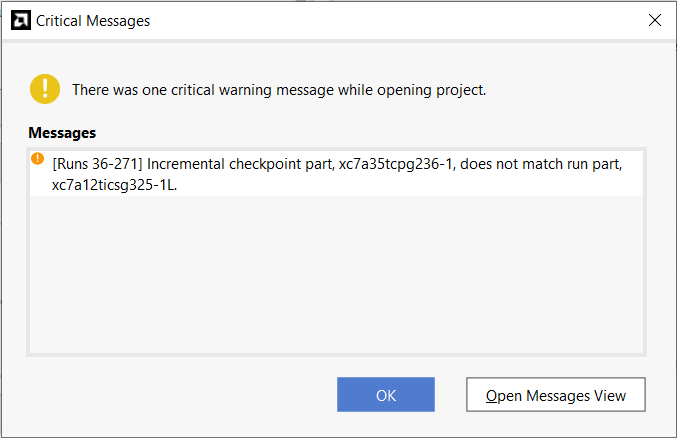
\includegraphics[width=0.48\textwidth]{err1.png}}
	\hfill
	\subfloat[Error]  {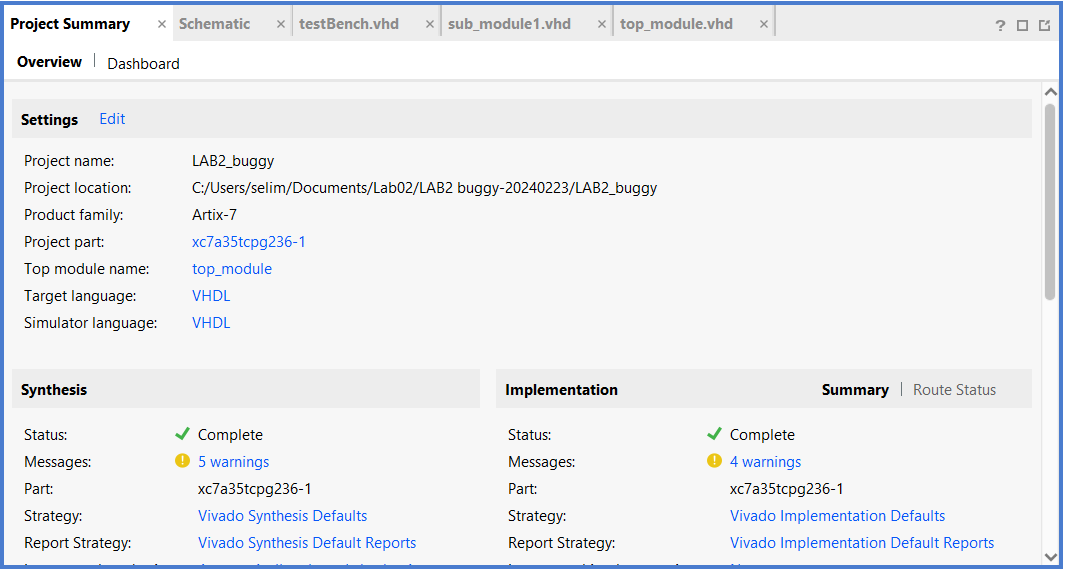
\includegraphics[width=0.48\textwidth]{fix1.png}}
	\caption{}
	\label{fig:err1}
\end{figure}


\subsection{Error Two}

Then, upon attempting to synthesize the project, another error popped up, which was fixed by correcting "s\_ouput\_1" to "s\_ouput\_1" in top\_module.vhd, as shown in figure \ref{fig:err2}.

\begin{figure}
	\centering
	\subfloat[Message]{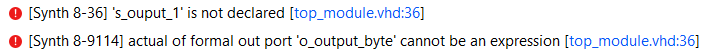
\includegraphics[width=0.48\textwidth]{err2.png}}
	\hfill
	\subfloat[Error]  {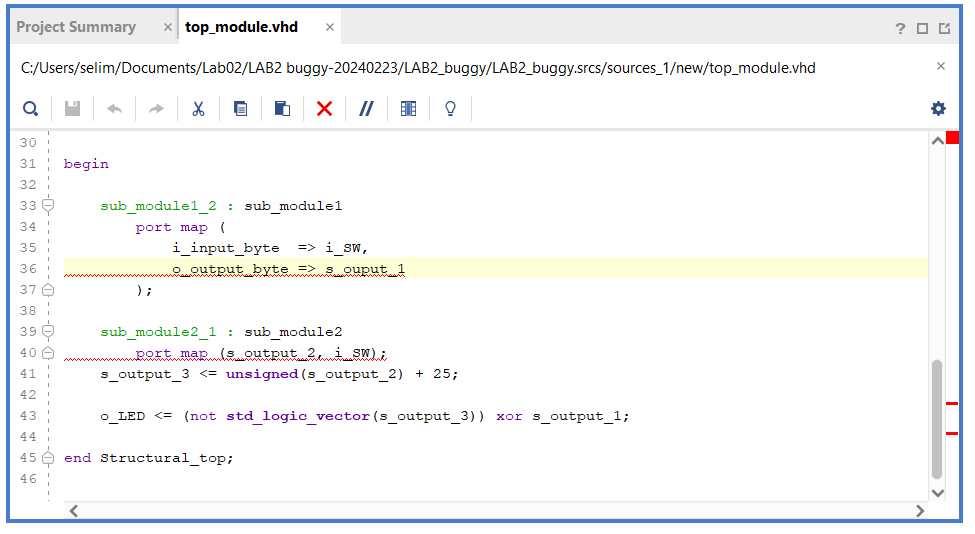
\includegraphics[width=0.48\textwidth]{fix2.png}}
	\caption{}
	\label{fig:err2}
\end{figure}

\subsection{Error Three}

Next, another error in the same file was found, which was fixed by swapping the places of "s\_output\_2" and "i\_SW", as shown in figure \ref{fig:err3}.

\begin{figure}
	\centering
	\subfloat[Message]{
\includegraphics[width=0.48\textwidth]{err3.png}}
	\hfill
	\subfloat[Error]  {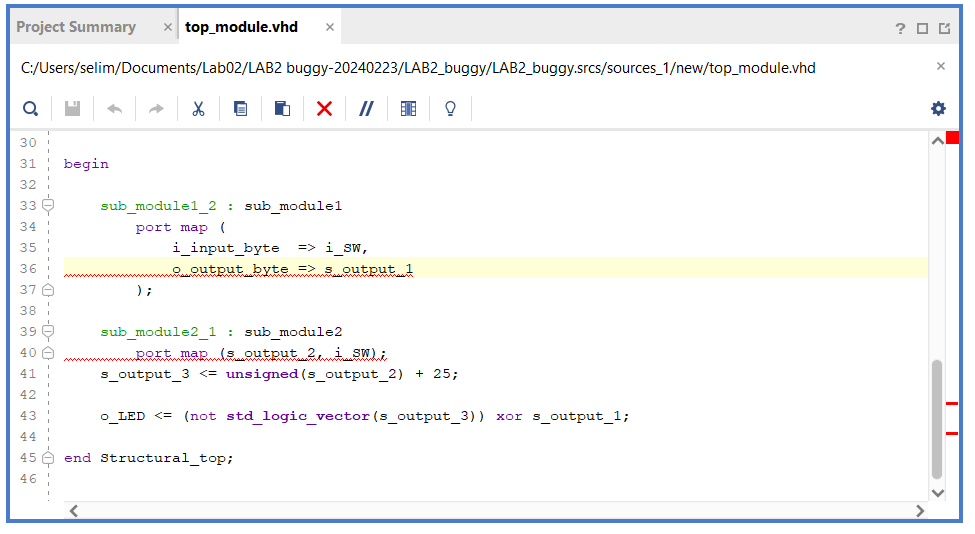
\includegraphics[width=0.48\textwidth]{fix3.png}}
	\caption{}
	\label{fig:err3}
\end{figure}

\subsection{Error Four}

\begin{wrapfigure}{r}{0.48\textwidth}
\vspace{-2cm}
	\centering
	\subfloat[Message]{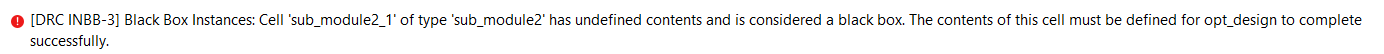
\includegraphics[width=0.48\textwidth]{err4.png}}
	\\
	\subfloat[Error]  {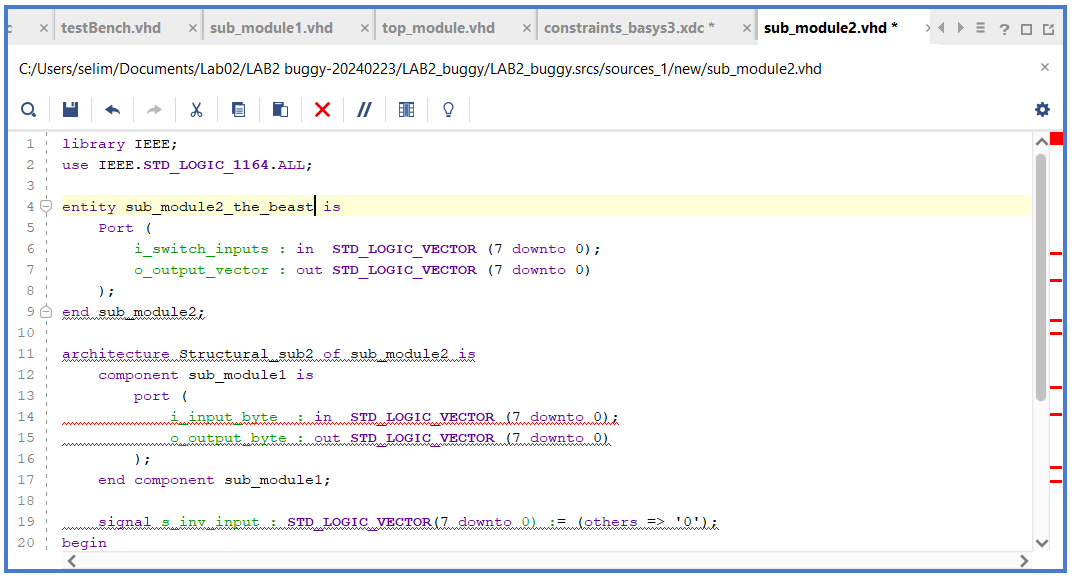
\includegraphics[width=0.48\textwidth]{fix4.png}}
	\caption{}
	\label{fig:err4}
\end{wrapfigure}

Then, the project synthesized successfully but another error occurred while implementation, which is then fixed by replacing "sub\_module2\_the\_beast"s with "sub\_module2" in sub\_module2.vhd, as seen in figure \ref{fig:err4}.

\subsection{Error Five and Six}

\begin{wrapfigure}{r}{0.48\textwidth}
\vspace{-5cm}
	\centering
	\subfloat[Message]{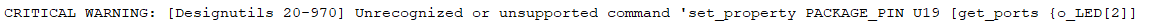
\includegraphics[width=0.48\textwidth]{err5.png}}
	\\
	\subfloat[Error 1]  {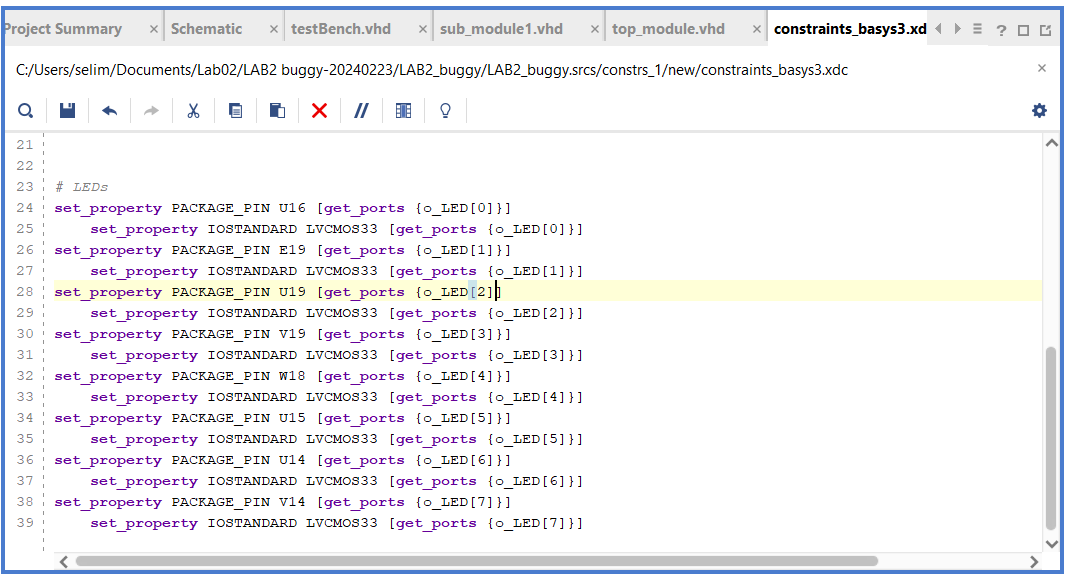
\includegraphics[width=0.48\textwidth]{fix5.png}}
	\caption{}
	\label{fig:err5}
\end{wrapfigure}

Afterwards, the project could be implemented but two other errors were found while bit streaming.
One of these errors was \\ fixed by adding the missing "\}", and the \\ other one by swapping places of "V14" \\ and "U16" in contraints\_basys3.xdc, as all \\ shown in figure \ref{fig:err5}b.

Finally after fixing all of the errors, the project is synthesized, implemented, and bit-streamed.
Before the project was uploaded to the board, the logic gates in the circuit were selected to be XOR, XNOR, AND, because the author's ID was ending with a 2 (as requested in LAB2.pdf).

Afterwards, a test bench was written (provided in Appendix) and ran for the fixed VHDL code.
The test bench simulates the logic circuit by running it with every input bit combination sequentially, which yields a graph, as seen in figure \ref{fig:bsy-sim}b.

Relevant switches on the FPGA board were flipped, inputting the five different input bit combinations (00000000 to 00000100) one-by-one.
As a result, LEDs of the board, which are connected to the output bits of the circuit, turned on and off, according to the output of the logic circuit.
Output of the board is compared with 
The outputs of the same selected bit combinations are looked up in the simulation graph, and are compared with the outputs of the FPGA board, as shown in figure \ref{fig:bsy-sim}.

\begin{figure}
	\centering
	\subfloat[Board 00000000]{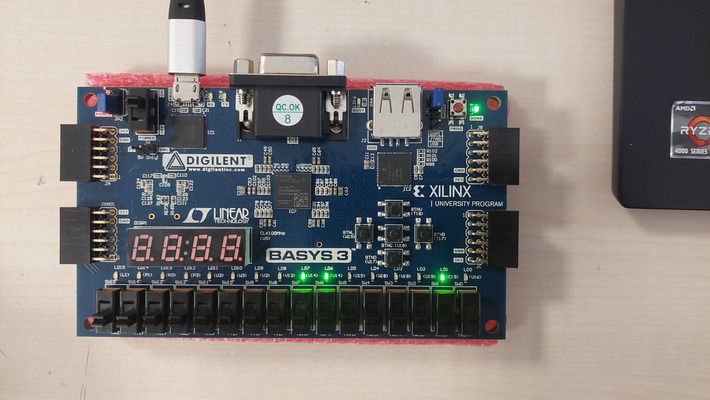
\includegraphics[width=0.48\textwidth]{bsy0.png}}
	\hfill                        
	\subfloat[Simulation 00000000]{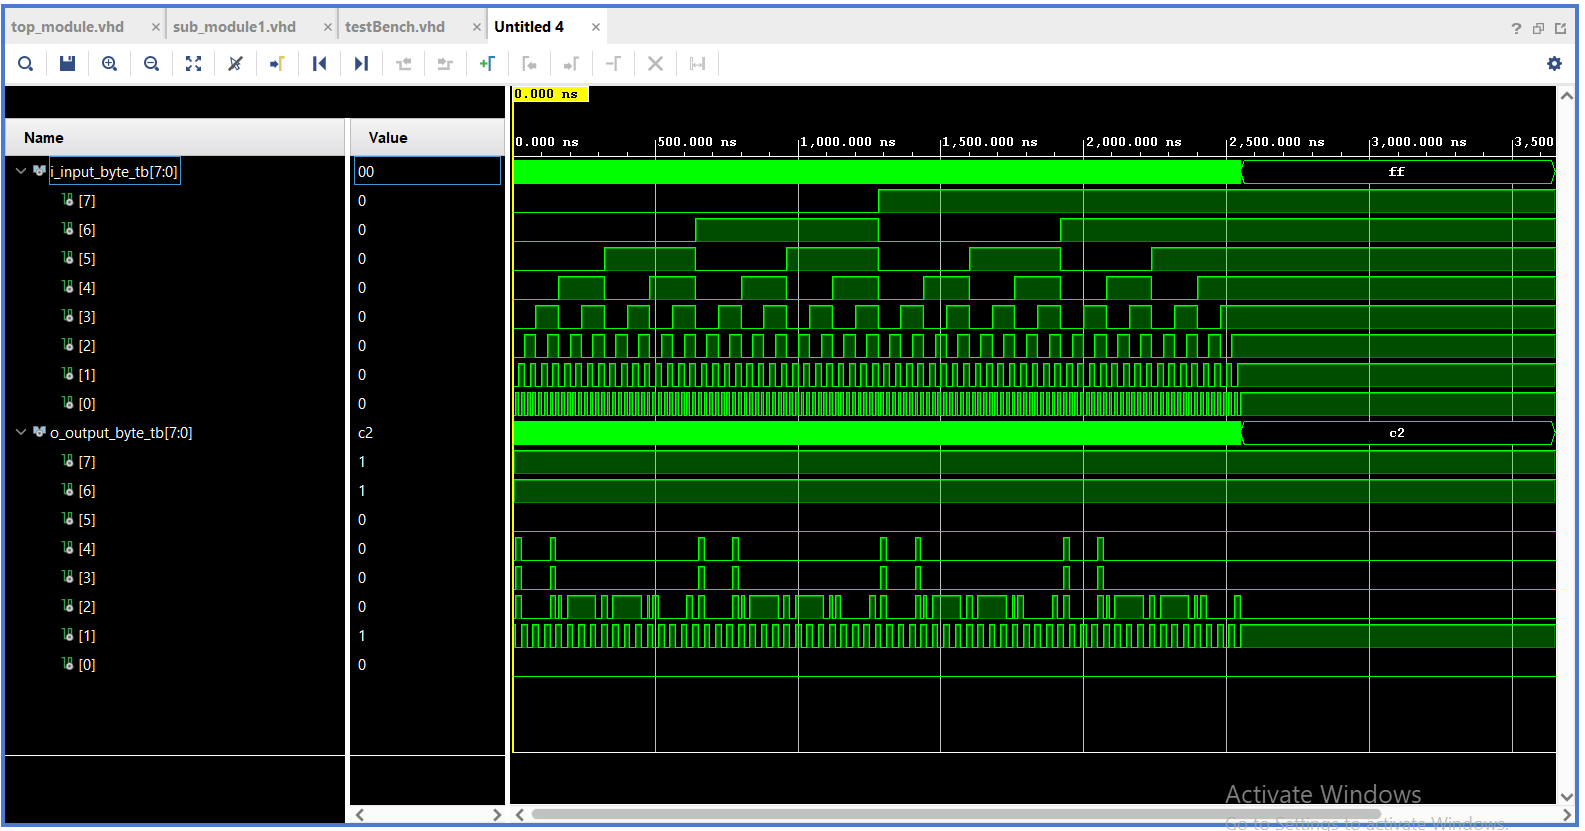
\includegraphics[width=0.48\textwidth]{sim0.png}}
	\\
	\subfloat[Board 00000001]{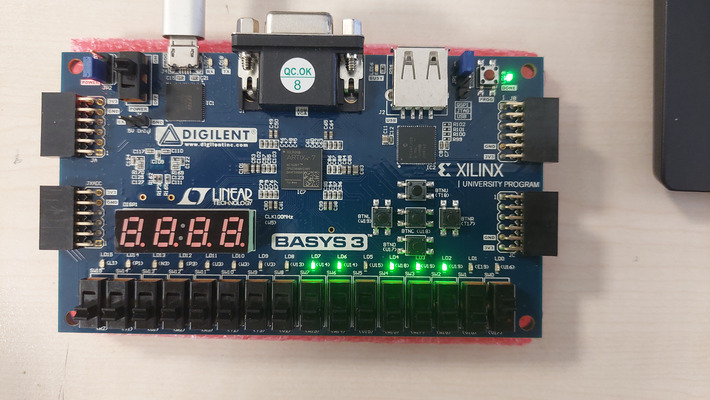
\includegraphics[width=0.48\textwidth]{bsy1.png}}
	\hfill                        
	\subfloat[Simulation 00000001]{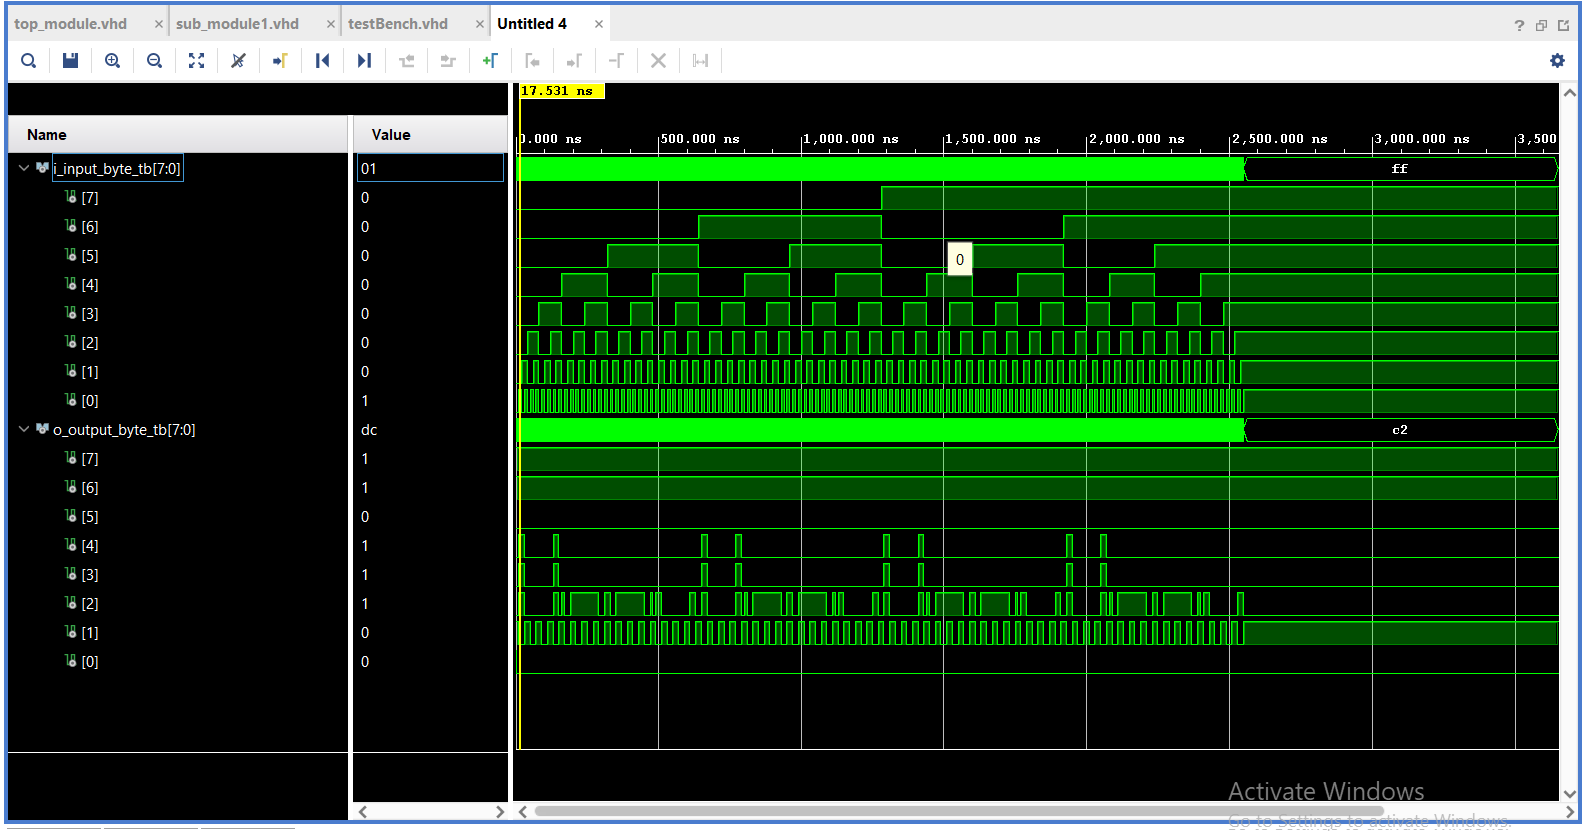
\includegraphics[width=0.48\textwidth]{sim1.png}}
	\\                            
	\subfloat[Board 00000010]{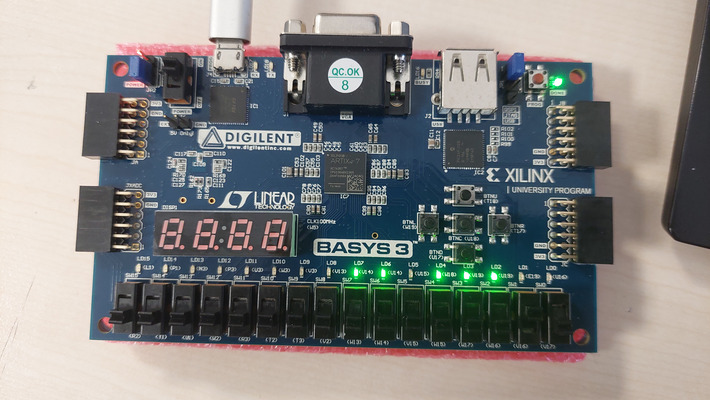
\includegraphics[width=0.48\textwidth]{bsy2.png}}
	\hfill                        
	\subfloat[Simulation 00000010]{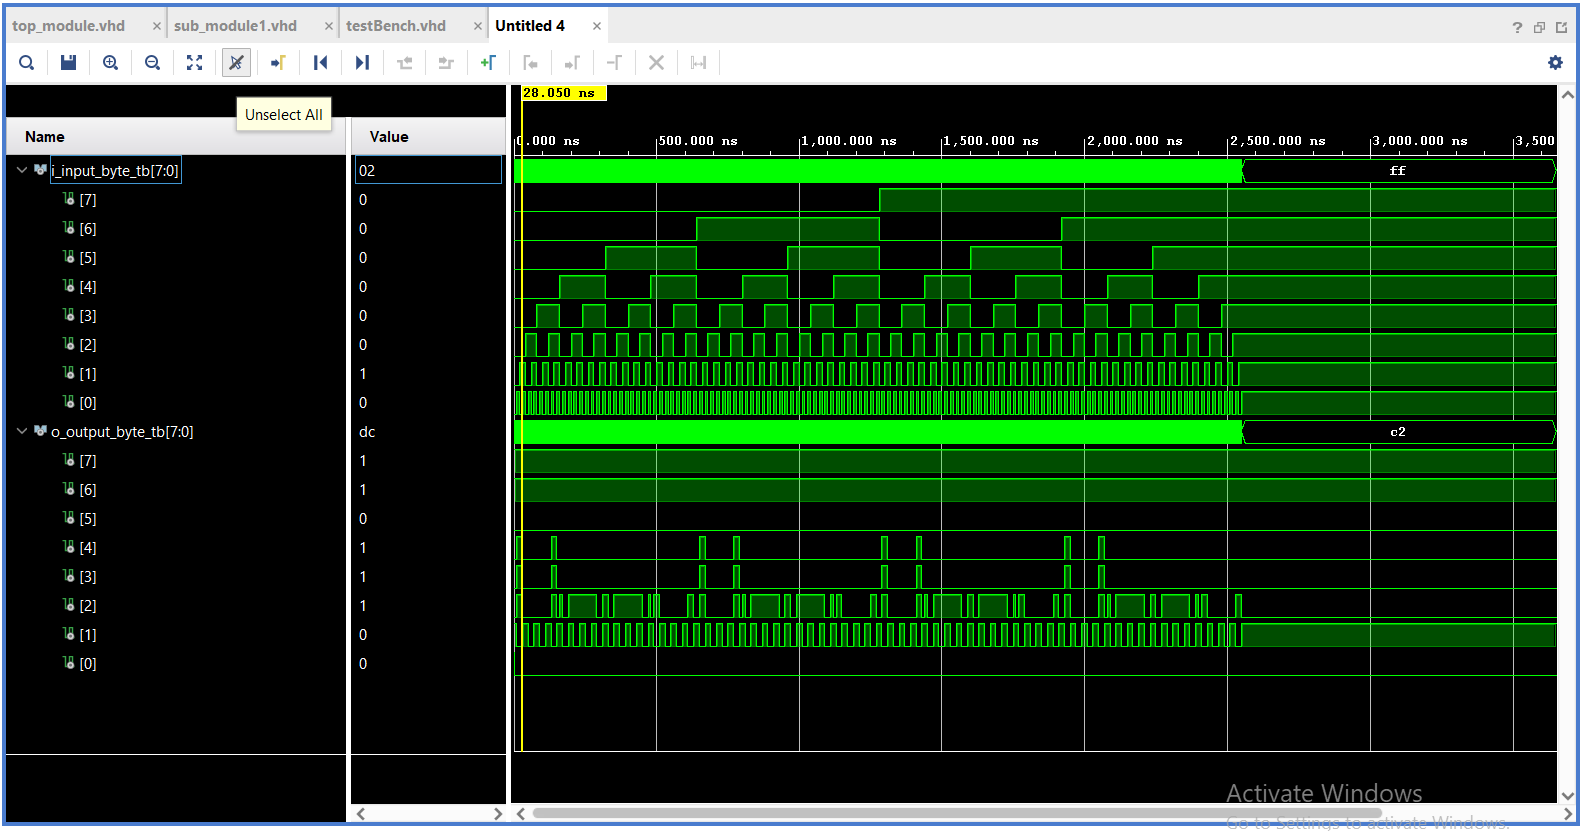
\includegraphics[width=0.48\textwidth]{sim2.png}}
	\\                            
	\subfloat[Board 00000011]{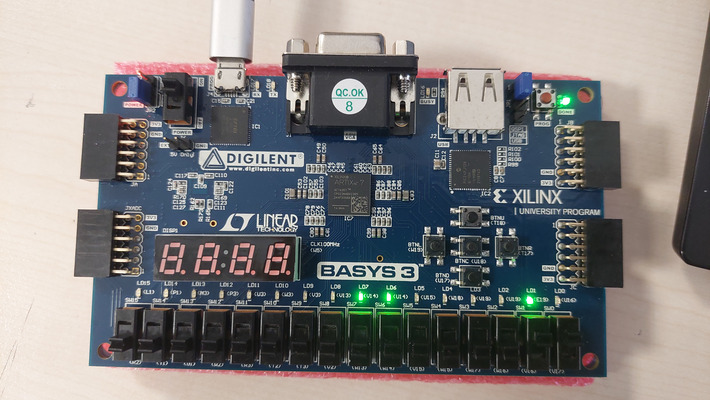
\includegraphics[width=0.48\textwidth]{bsy3.png}}
	\hfill                        
	\subfloat[Simulation 00000011]{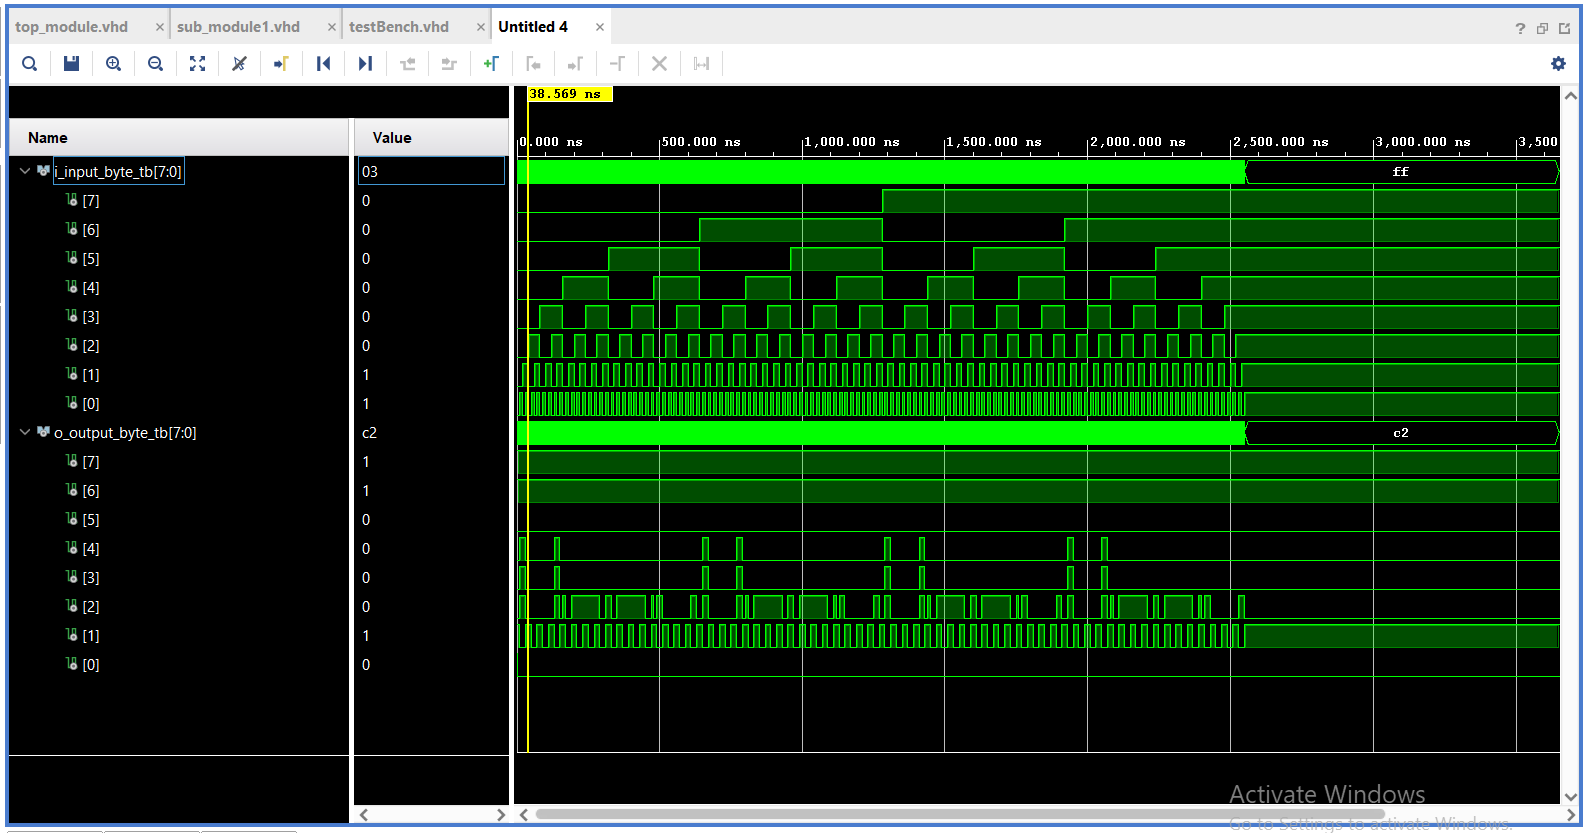
\includegraphics[width=0.48\textwidth]{sim3.png}}
	\\                            
	\subfloat[Board 00000100]{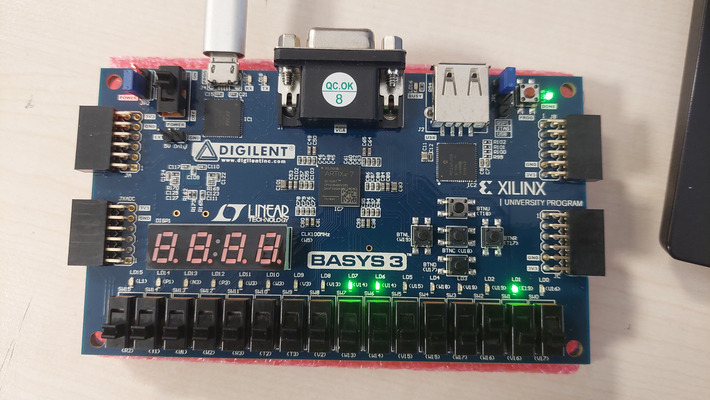
\includegraphics[width=0.48\textwidth]{bsy4.png}}
	\hfill                        
	\subfloat[Simulation 00000100]{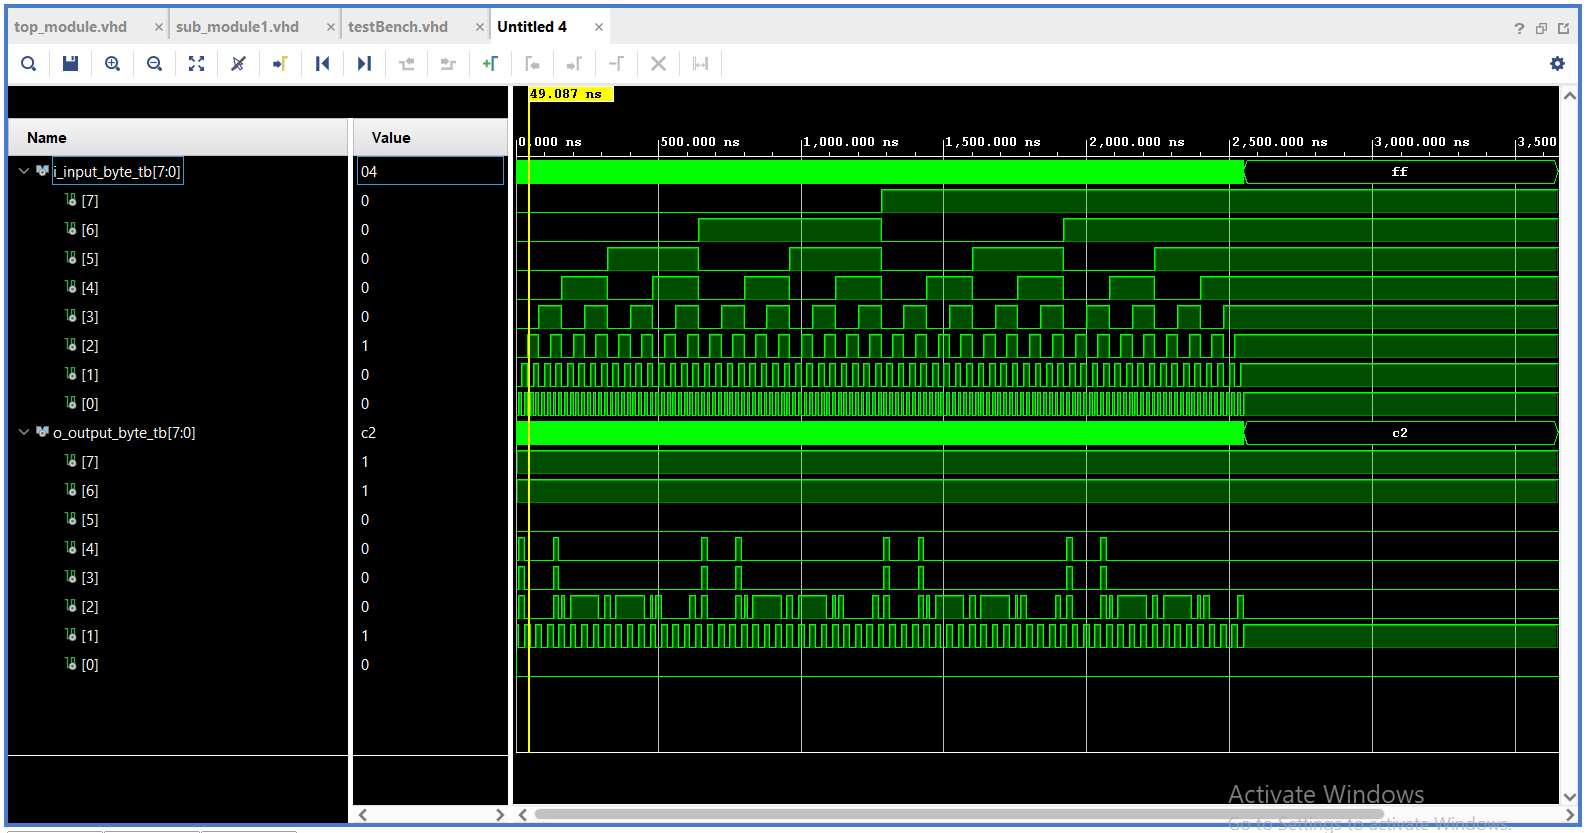
\includegraphics[width=0.48\textwidth]{sim4.png}}
	\caption{}
	\label{fig:bsy-sim}
\end{figure}
\newpage
\section{Schematics}

\begin{figure}[!h]
	\centering
	\subfloat[RTL]{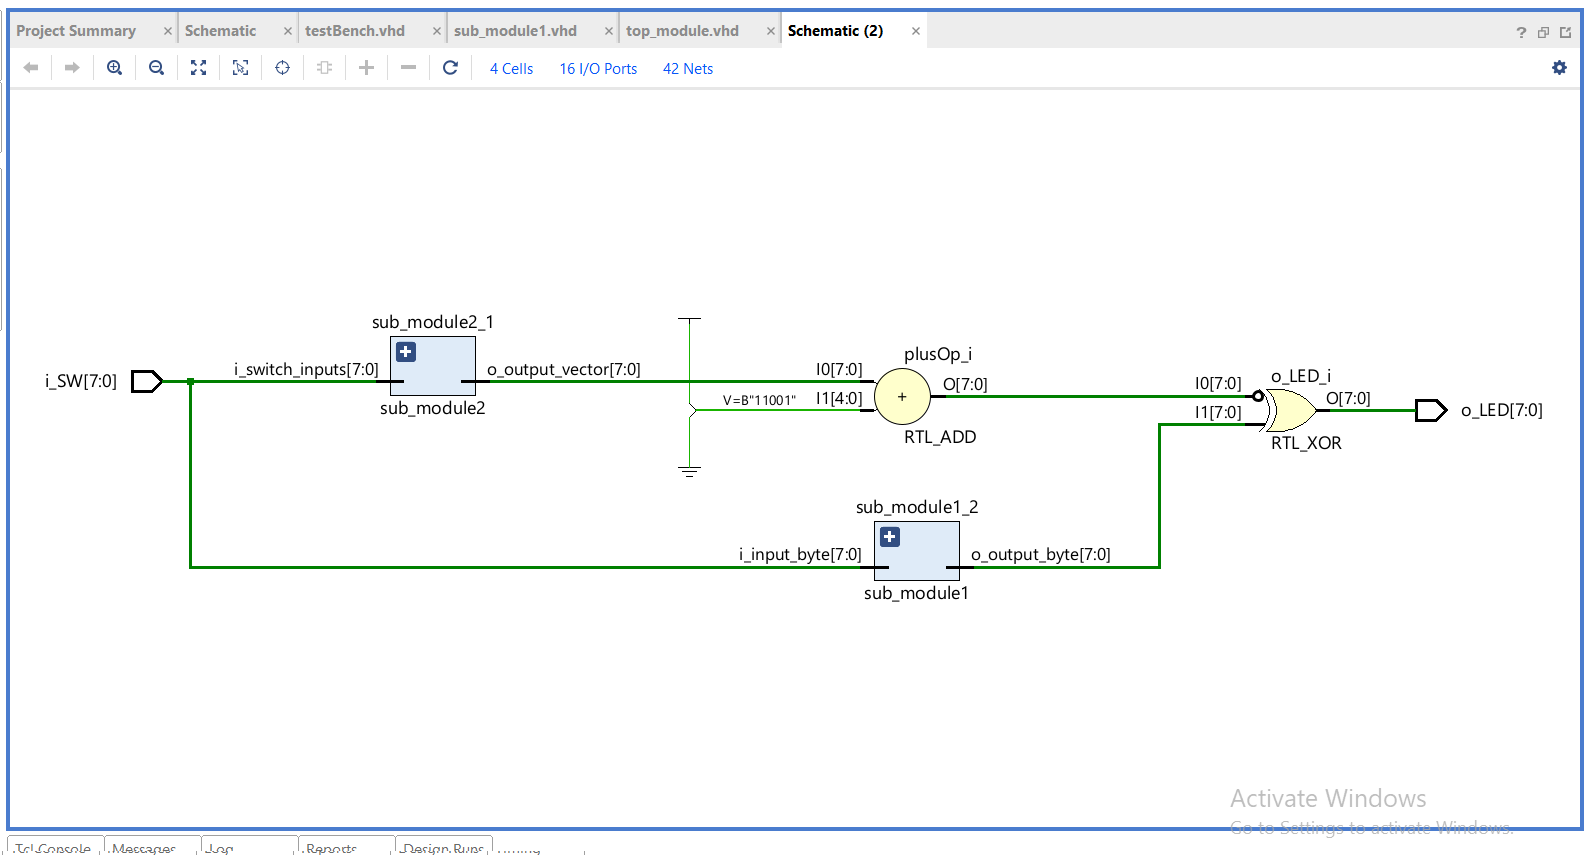
\includegraphics[width=\textwidth]{sch1.png}}
	\\                        
	\subfloat[Synthesized]{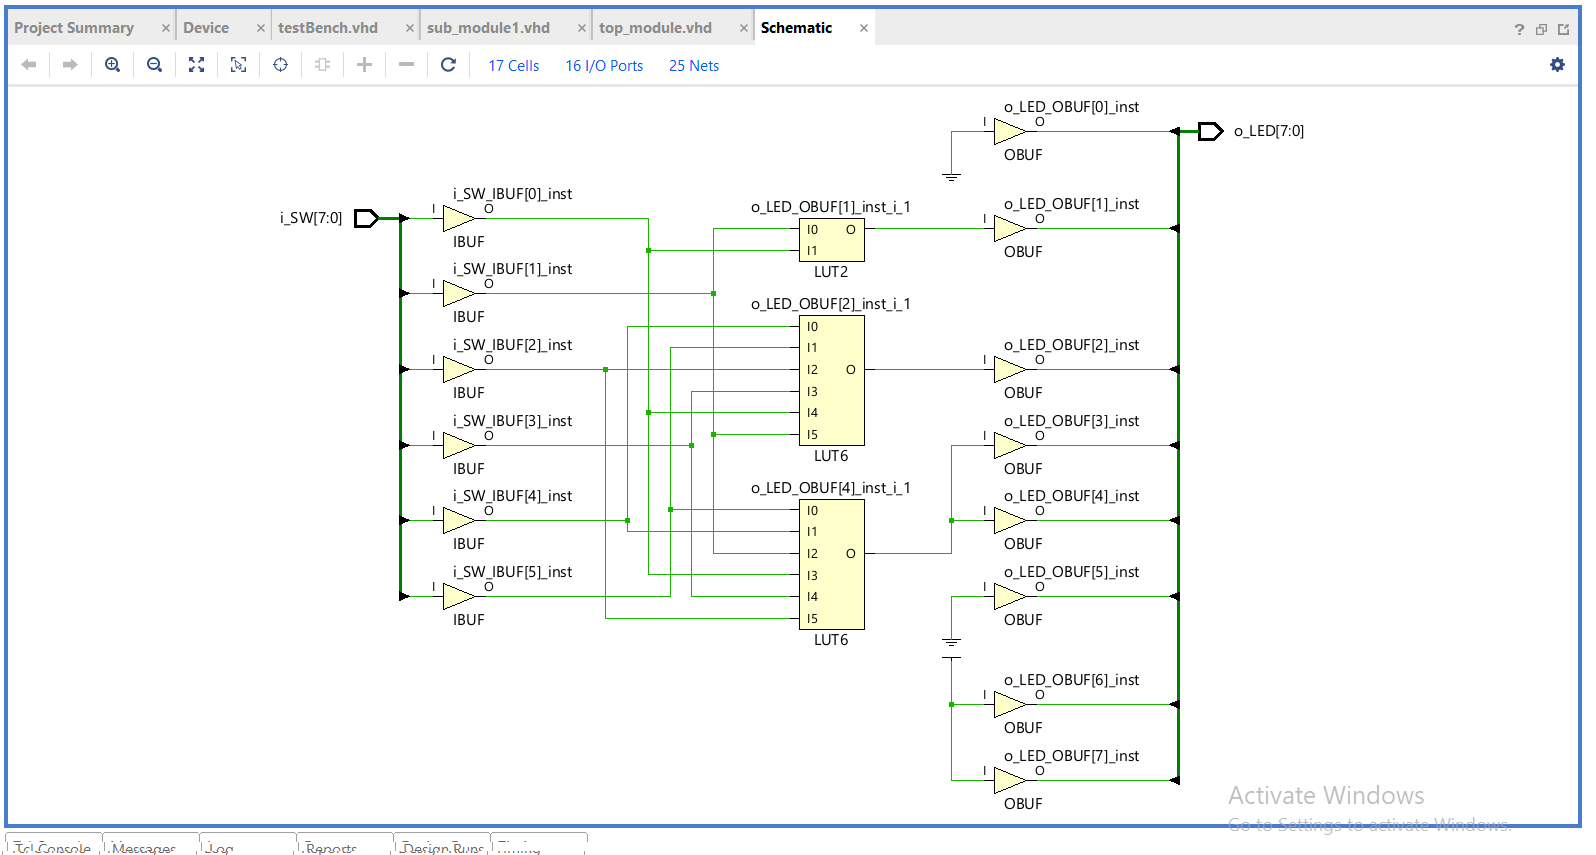
\includegraphics[width=0.48\textwidth]{sch2.png}}
	\hfill
	\subfloat[Implemented]{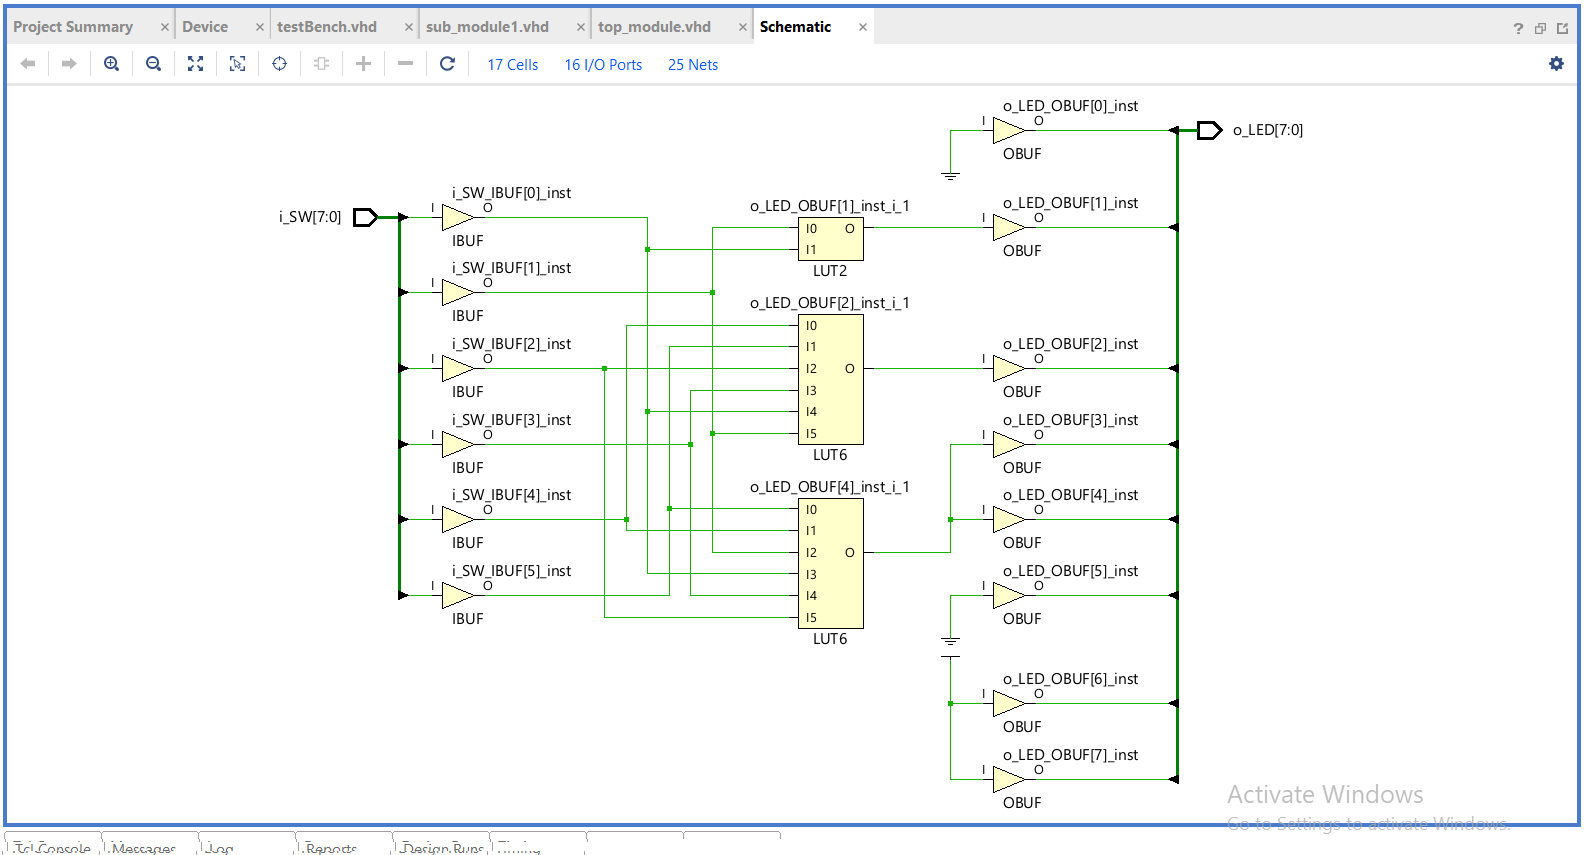
\includegraphics[width=0.48\textwidth]{sch3.png}}
	\caption{Schematics}
	\label{fig:schs}
\end{figure}

Figure \ref{fig:schs} shows the three schematics in Vivado.
The RTL schematic shows the design at a generally higher abstraction level, and more useful to understand the overall structure of the project.
The Synthesized and Implemented schematics, both showing the same image, shows a very detailed implementation of the circuit, close to the codes uploaded to the FPGA.
The Synthesized and Implemented schematics are greatly optimized by Vivado, so that they use lookup tables (LUT).

\section{Conclusion}
In this lab, we learned and practiced how to effectively use the Vivado software to design, implement and simulate VHDL code for an FPGA board.
Doing so, we did research about what constraint and testbench are and how to define io for a VHDL module.
In order to fix the broken code, we read and studied the given code, compared it to tutorials, and found a chance to practice our VHDL skills.

\appendix

\section{sub\_module1.vhd}
\lstinputlisting[language=VHDL]{code/sub\_module1.vhd}

\section{sub\_module2.vhd}
\lstinputlisting[language=VHDL]{code/sub\_module2.vhd}

\section{top\_module.vhd}
\lstinputlisting[language=VHDL]{code/sub\_module2.vhd}

\section{testBench.vhd}
\lstinputlisting[language=VHDL]{code/testBench.vhd}

\section{constraints\_basys3.xdc}
\lstinputlisting{code/sub\_module2.vhd}
\end{document}
